\documentclass[12pt,fleqn]{article}
\usepackage[margin=1in,top=1in,bottom=1in]{geometry}
\usepackage{mathtools}
\usepackage{longtable}
\usepackage{enumitem}
%\usepackage{hyperref}
\usepackage[dvips]{graphics}
\usepackage[table]{xcolor}
\usepackage{amssymb}
%\usepackage{subfig}
\usepackage{booktabs}
\usepackage{tikz}
\usepackage{subcaption}

\usepackage[normalem]{ulem}

\usepackage{multicol}
\usepackage{txfonts}
%\usepackage{amsfonts}

%%%%%%%%%% bibliography stuff %%%%%%%%%%%%%
\usepackage[numbers]{natbib}
\bibliographystyle{abbrvnat}
%\usepackage{natbib}
%\bibliographystyle{/Users/tonhauser.1/Library/Latex/cslipubs-natbib}

\setlength{\bibhang}{0.5in}
\setlength{\bibsep}{0mm}
%\bibpunct[:]{(}{)}{;}{a}{,}{,}
%%%%%%%%%%%%%%%%%%%%%%%%%%%%%%%

\usepackage{wrapfig}

\usepackage{gb4e}
%\usepackage{/Users/judith/Library/Latex/drs}
%\usepackage{/Users/judith/Library/Latex/avm}
\usepackage[all]{xy}
\usepackage{rotating}
\usepackage{tipa}
\usepackage{multirow}
\usepackage{authblk}
\usepackage{adjustbox}
\usepackage{array}

\usepackage{titlesec}
\titleformat*{\section}{\bfseries\footnotesize}
 
\setlength{\parindent}{.3cm}
\setlength{\parskip}{0ex}

\renewcommand\figurename{Fig.}

\newcommand{\yi}{\'{\symbol{16}}}
\newcommand{\nasi}{\~{\symbol{16}}}
\newcommand{\hina}{h\nasi na}
\newcommand{\ina}{\nasi na}

\exewidth{(\thexnumi)}

\newcommand{\citepos}[1]{\citeauthor{#1}'s \citeyear{#1}}

\newcommand{\6}{\mbox{$[\hspace*{-.6mm}[$}} 
\newcommand{\9}{\mbox{$]\hspace*{-.6mm}]$}}
\newcommand{\sem}[2]{\6#1\9$^{#2}$}
\renewcommand{\ni}{\~{\i}}

\newcommand{\jt}[1]{\textbf{\color{blue}JT: #1}}


\setlength{\belowcaptionskip}{-10pt}


 \begin{document}
  
\begin{center}
{\bf An empirical challenge to the categorical notion of factivity}

Judith Tonhauser (OSU / Stuttgart U) \& Judith Degen (Stanford U) 
\end{center}

\vspace*{-.19cm}

%\begin{wrapfigure}{r}{0.32\textwidth}
%\centering
%  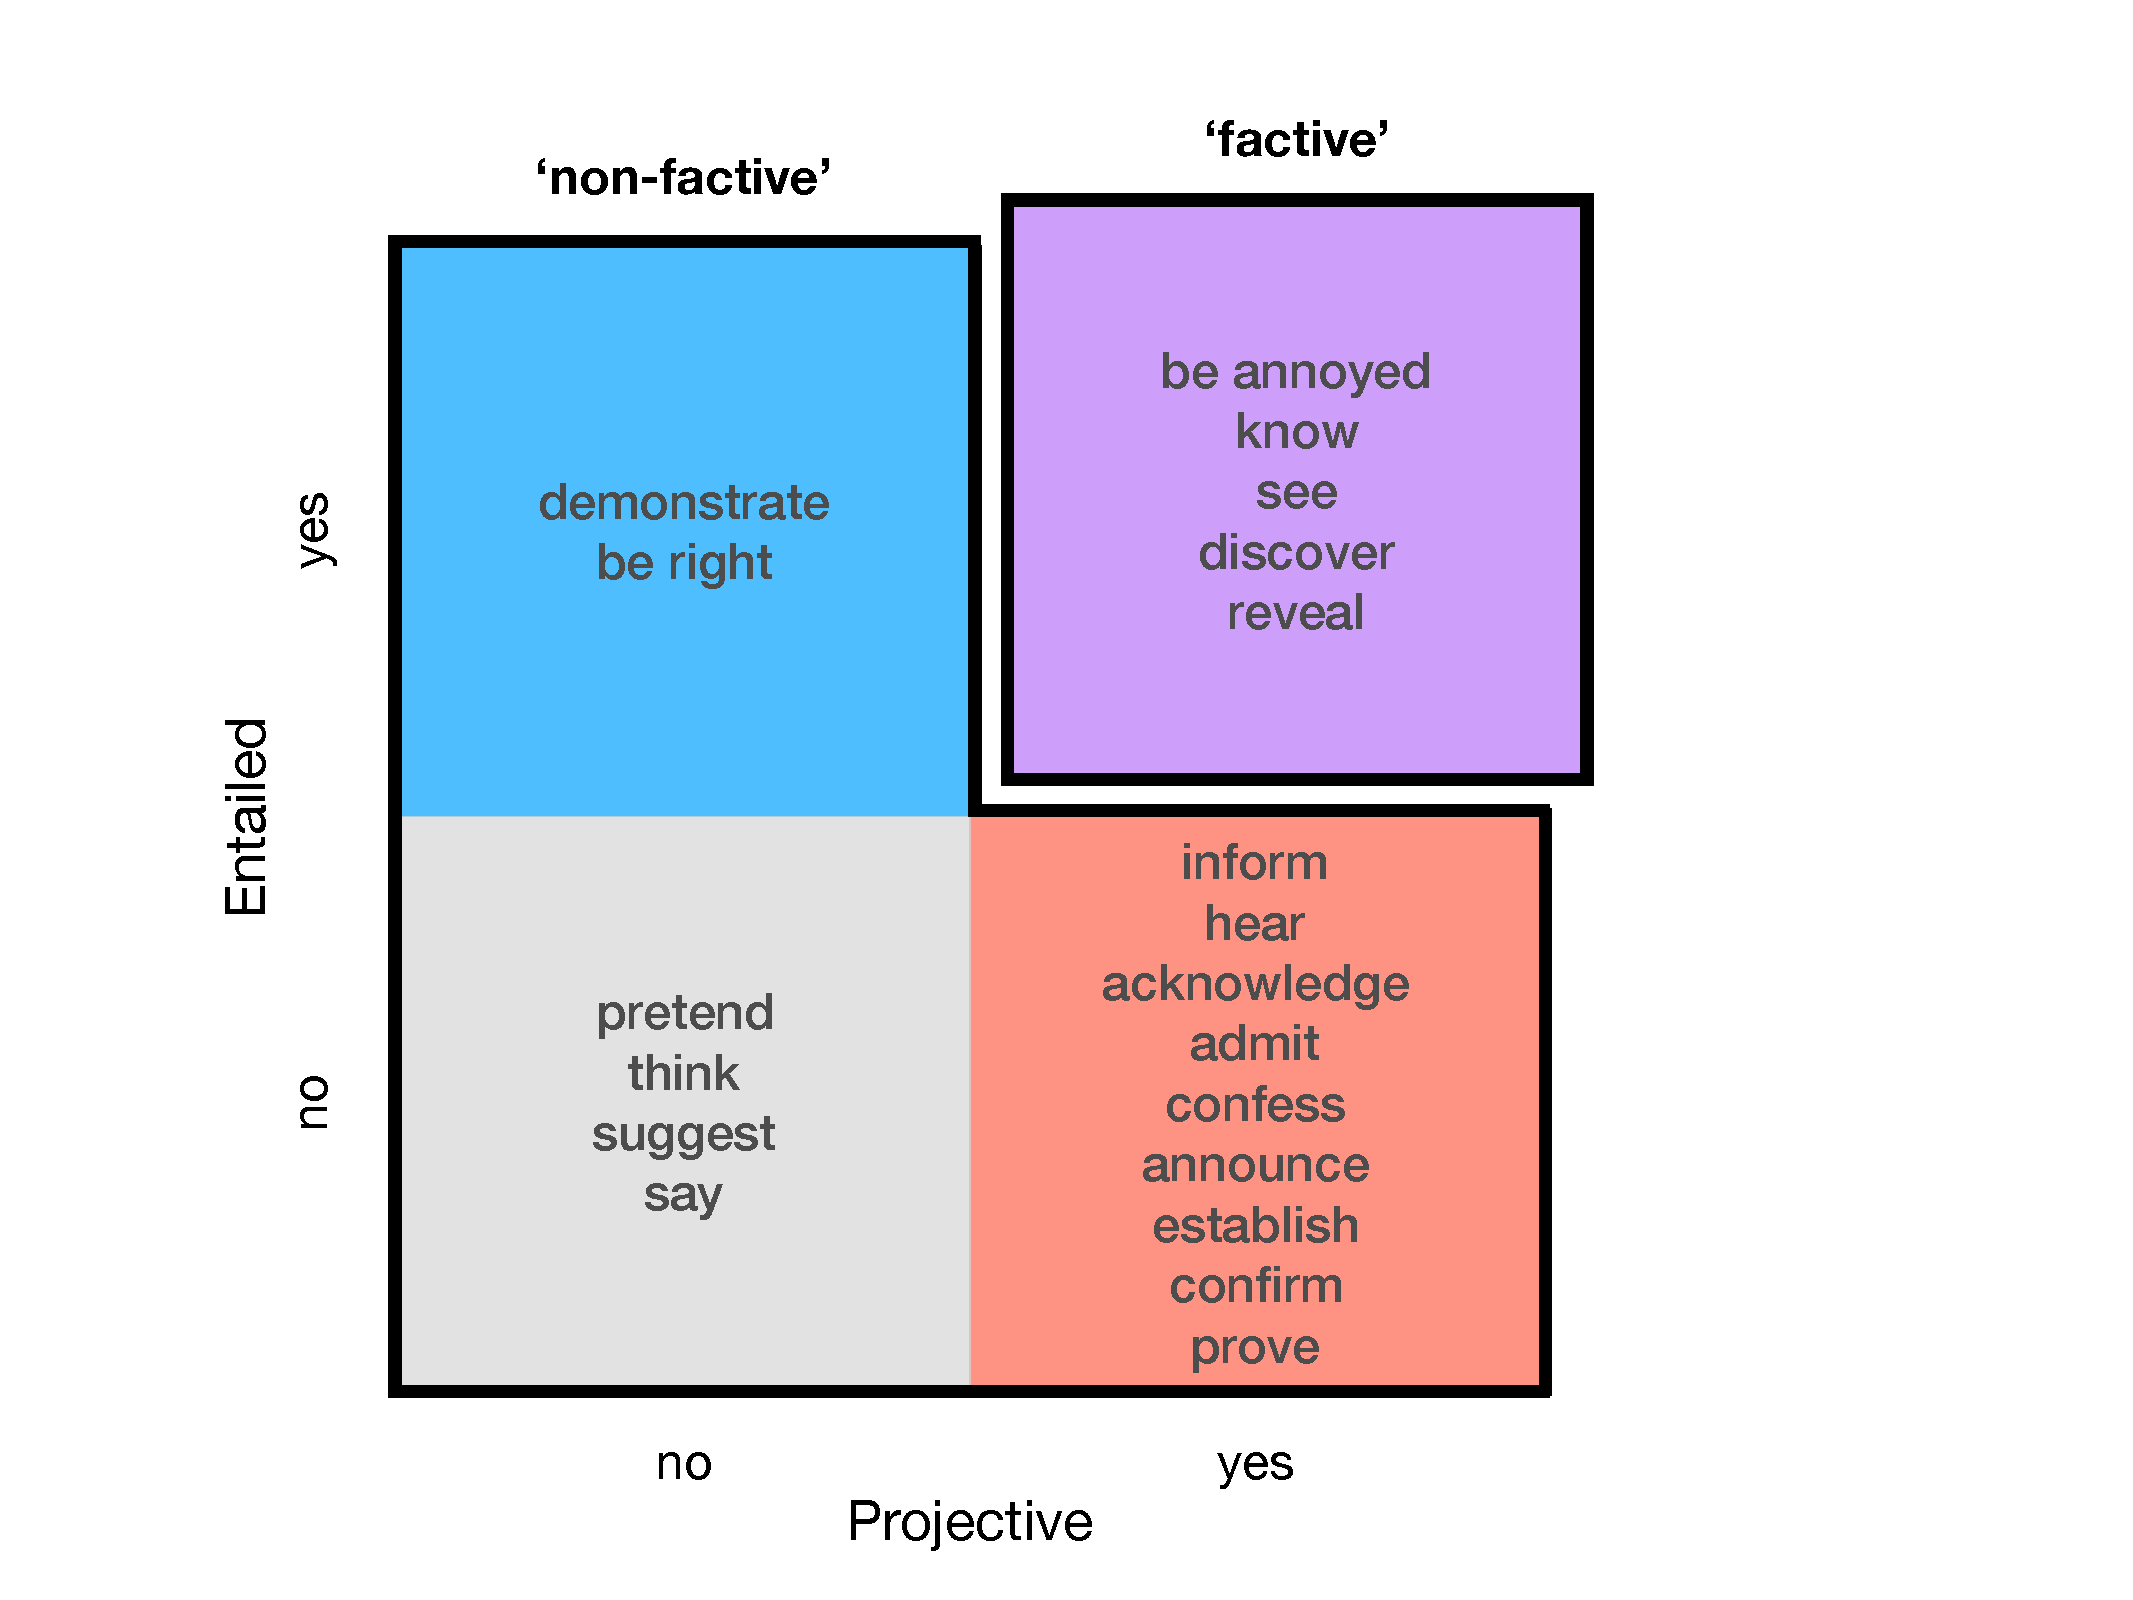
\includegraphics[trim={3.5cm 1cm 7cm 2cm},clip,width=.27\paperwidth]{../paper/figures/categorization}
%  \caption{Standard classification of 20 English predicates}\label{f-cat}
%\end{wrapfigure} 

\noindent
Projection analyses have largely limited their attention to `factive' predicates, like {\em know}, to the exclusion of `non-factive' ones, like {\em think}  (e.g., \cite{heim83,vds92,abrusan2011,abrusan2016,romoli2015,best-question}). This limitation is motivated by the long-standing and widely-held assumption that `factive' predicates are empirically distinct from `non-factive' ones (see, e.g., \cite{karttunen71b,kiparsky-kiparsky71} and much literature thereafter): the content of the complement (CC) of a `factive' predicate is taken to be both projective and entailed, whereas `non-factive' CCs  are taken to not be both projective and entailed  (e.g., \cite{gazdar79a}, \cite{ccmg90}, \cite{vds92},  \cite{schlenker10}, \cite{anand-hacquard2014}, \cite{spector-egre2015}). 

Despite the importance of the distinction between `factive' and `non-factive' predicates, the distinction has not been systematically investigated. Filling this lacuna is particularly pressing given that there is disagreement about which predicates are `factive'. For instance, \cite{schlenker10} assumed that {\em inform} is `factive', in contrast to \cite{anand-hacquard2014} who argued that \emph{inform}'s CC is not entailed. Similarly, emotive predicates like {\em be annoyed} are taken to be `factive' by some (e.g., \cite{gazdar79a,abrusan2011,anand-hacquard2014}) but not others (e.g., \cite{klein1975,giannakidou1998,schlenker2003,egre2008}). We report the results of two experiments designed to investigate the distinction by measuring projectivity and entailment for 20 predicates (see left panel of Fig.\ \ref{f-summary-categorical}). %{\bf maybe add question marks in the figure after the predicates where people have disagreements? be annoyed, inform, establish, hear)}

\noindent {\bf Exp.~1 (n=300):} Projectivity was measured with the `certain that' diagnostic (see also, e.g., \cite{tonhauser-salt26,tbd-variability}). Participants rated items like ``Helen asks: \emph{Did Amanda discover that Julian dances salsa?}'' for whether the speaker is certain about the CC (that Danny ate the last cupcake) on a sliding scale from \emph{no} to \emph{yes} (400 items total). Higher certainty ratings indicate greater projectivity.  

\noindent {\bf Exp.~2 (n=300):} Entailment was measured with the `inference' diagnostic: $p$ entails $q$ iff $q$ follows from $p$. %; under the `contradictoriness' diagnostic, $p$ entails $q$ iff $p$ {\em but not} $q$ is contradictory. 
Participants rated whether the CC follows for items like ``What is true: Amanda discovered that Julian dances salsa''; ratings were given on a sliding scale from \emph{no} to \emph{yes} (400 items total). Predicates were classified as entailing iff they were  indistinguishable from entailing controls. 

\noindent {\bf Results and discussion:} As shown in the right panel of Fig.\ \ref{f-summary-categorical}, the CCs of most of the predicates assumed to be `factive' (in purple) are entailed and highly projective, whereas those of predicates assumed to be `non-factive' (in grey) are not entailed and at most weakly projective. This finding is mostly in line with intuitions reported in the literature. However, because projectivity is observed to be a gradient property of utterance content (see also \cite{tbd-variability}), there is no non-arbitrary, binary division of predicates by projectivity. This finding challenges the assumed categorical distinction between \vspace{-1.15em}
\begin{wrapfigure}{r}{.77\textwidth}
\begin{subfigure}{.35\textwidth}
\centering
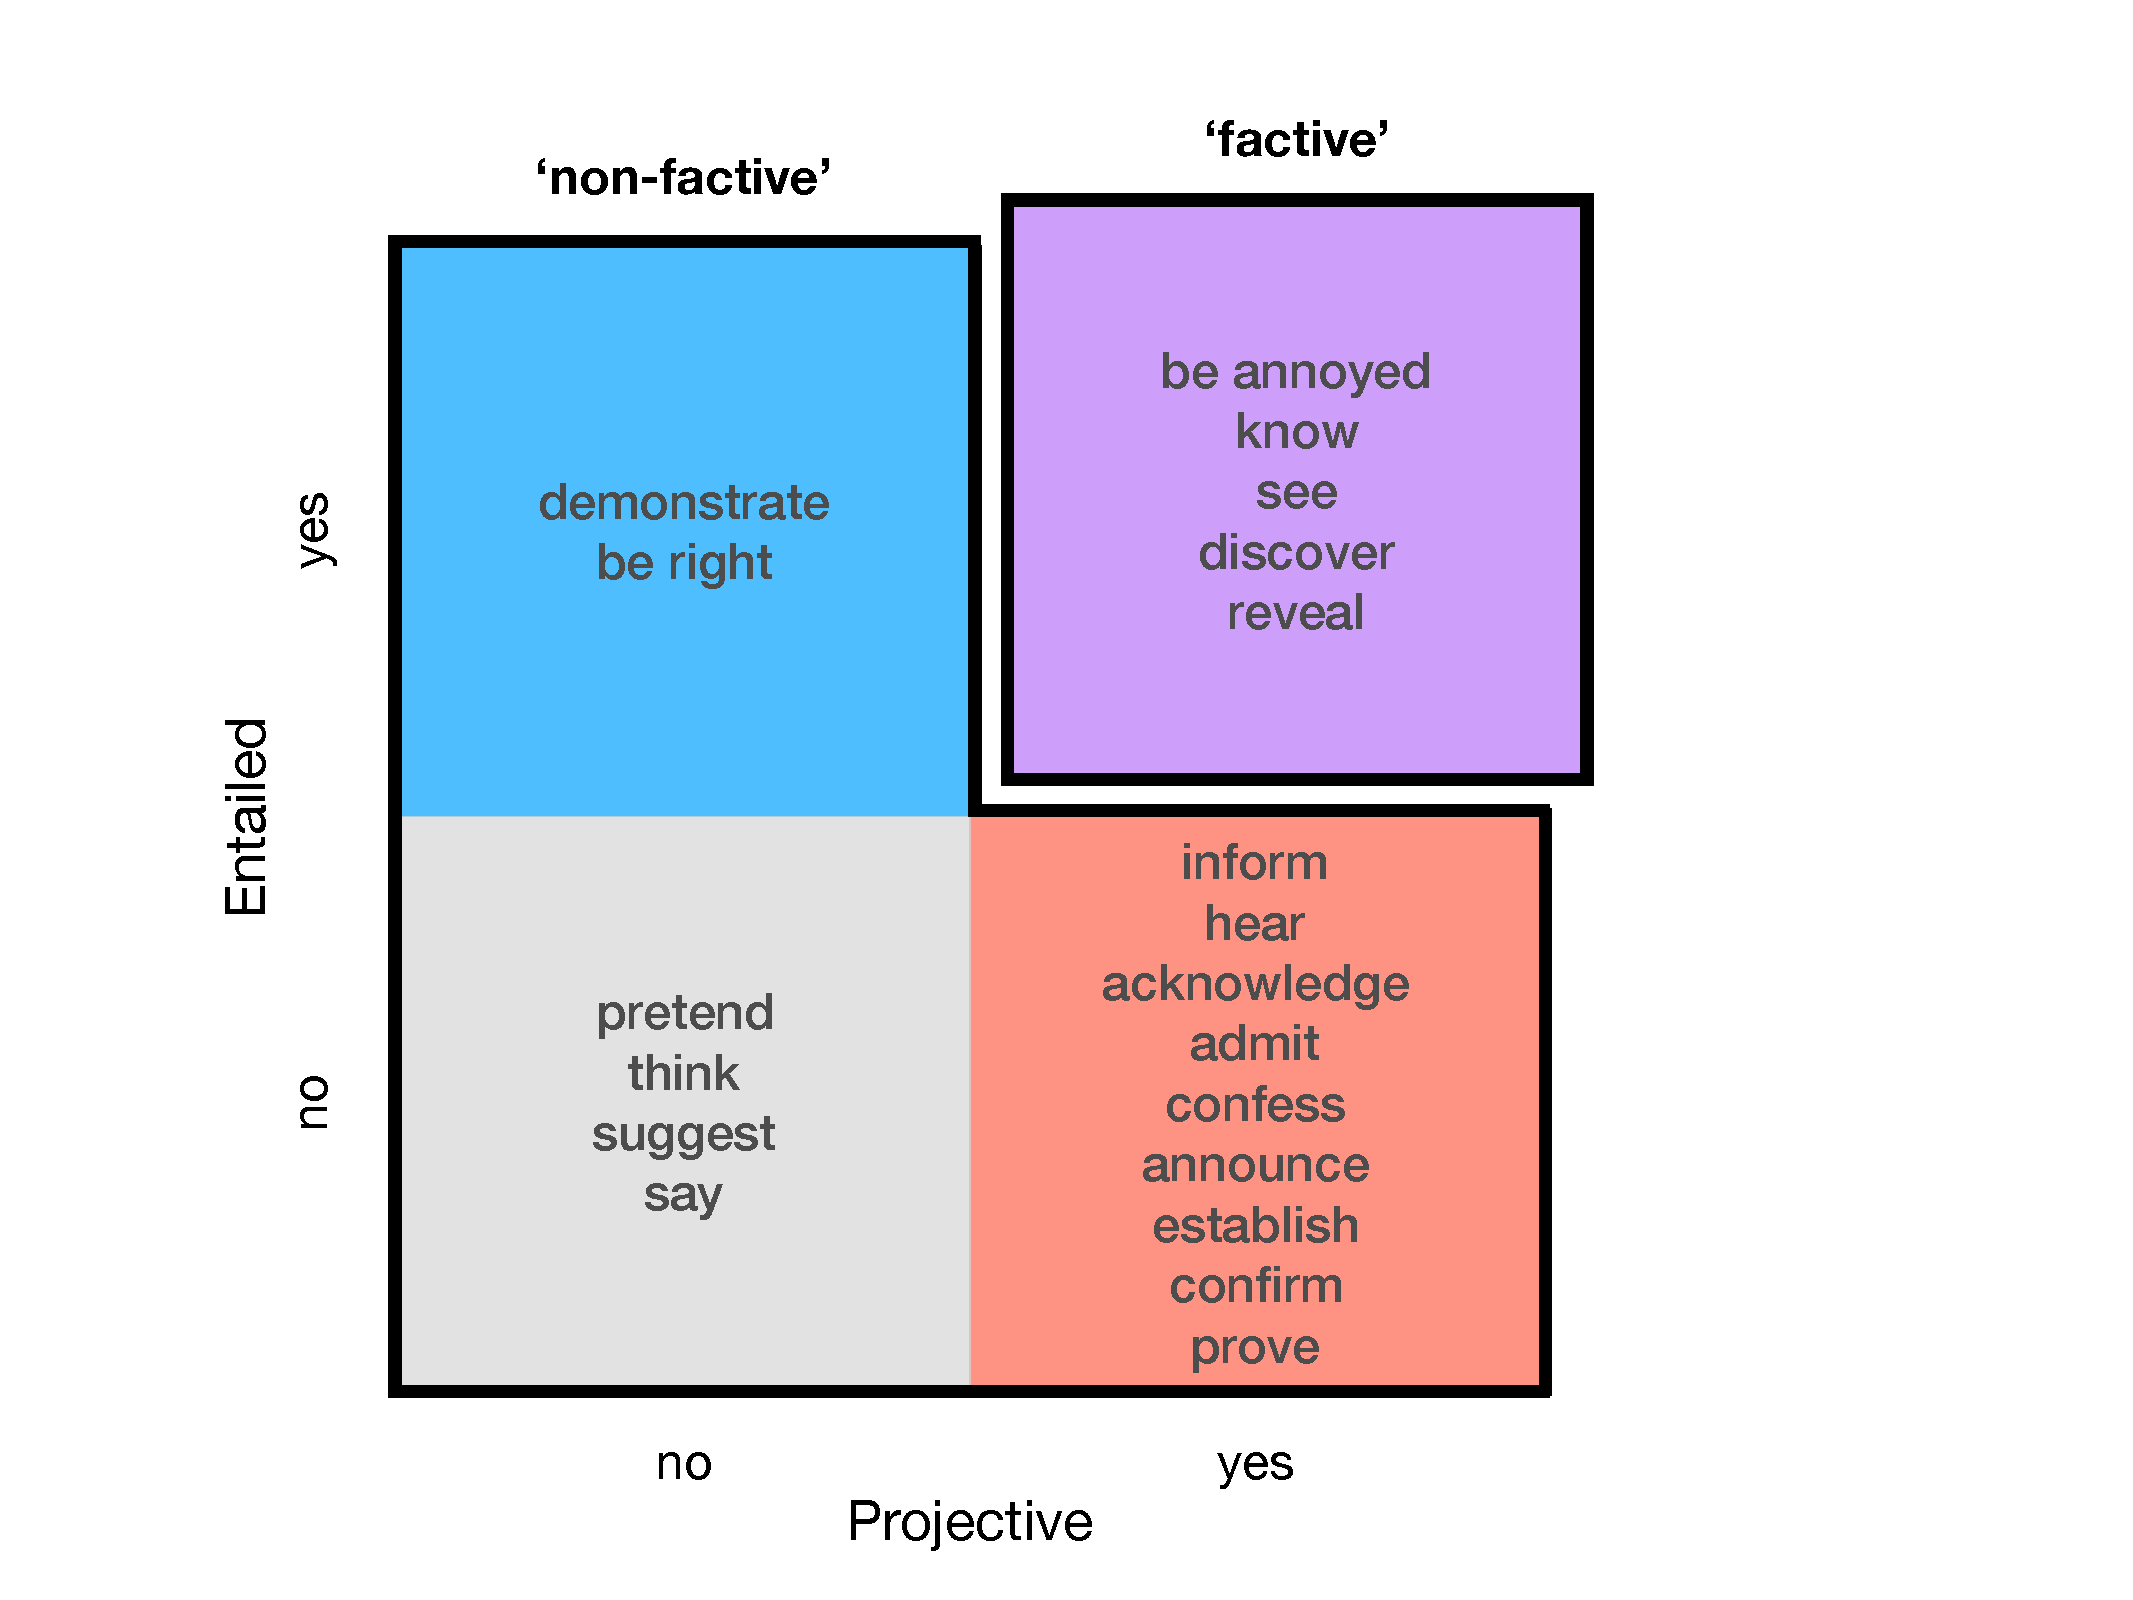
\includegraphics[width=.27\paperwidth]{../paper/figures/categorization}
%\caption{Assumed categorical classification}
\end{subfigure} %
\begin{subfigure}{.3\textwidth}
\centering
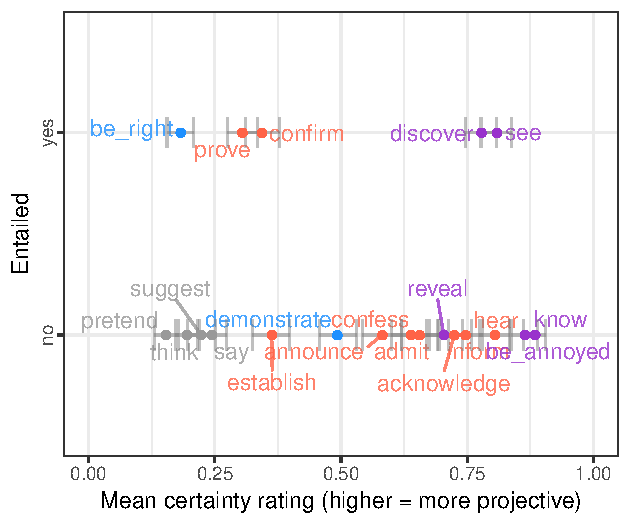
\includegraphics[width=.3\paperwidth]{../results/5-projectivity-no-fact/graphs/projection-by-inferenceEntailment}
%\caption{Experiment findings}
\end{subfigure}

\caption{Received categorical classification (left) vs.\ experimental results (right; entailment against mean certainty ratings) for 20 predicates.}\label{f-summary-categorical}

\end{wrapfigure}

\noindent
`factive' and `non-factive' predicates.  The finding that the CC of many `non-factives' is projective points to exciting, uncharted territory for future projection analyses. We also discuss issues with entailment diagnostics and suggest that research on entailment needs to consider the pragmatics of entailment judgments (see also \cite{demarneffe-etal2012}).

%\begin{figure}[h]
%
%\begin{subfigure}{.35\textwidth}
%\centering
%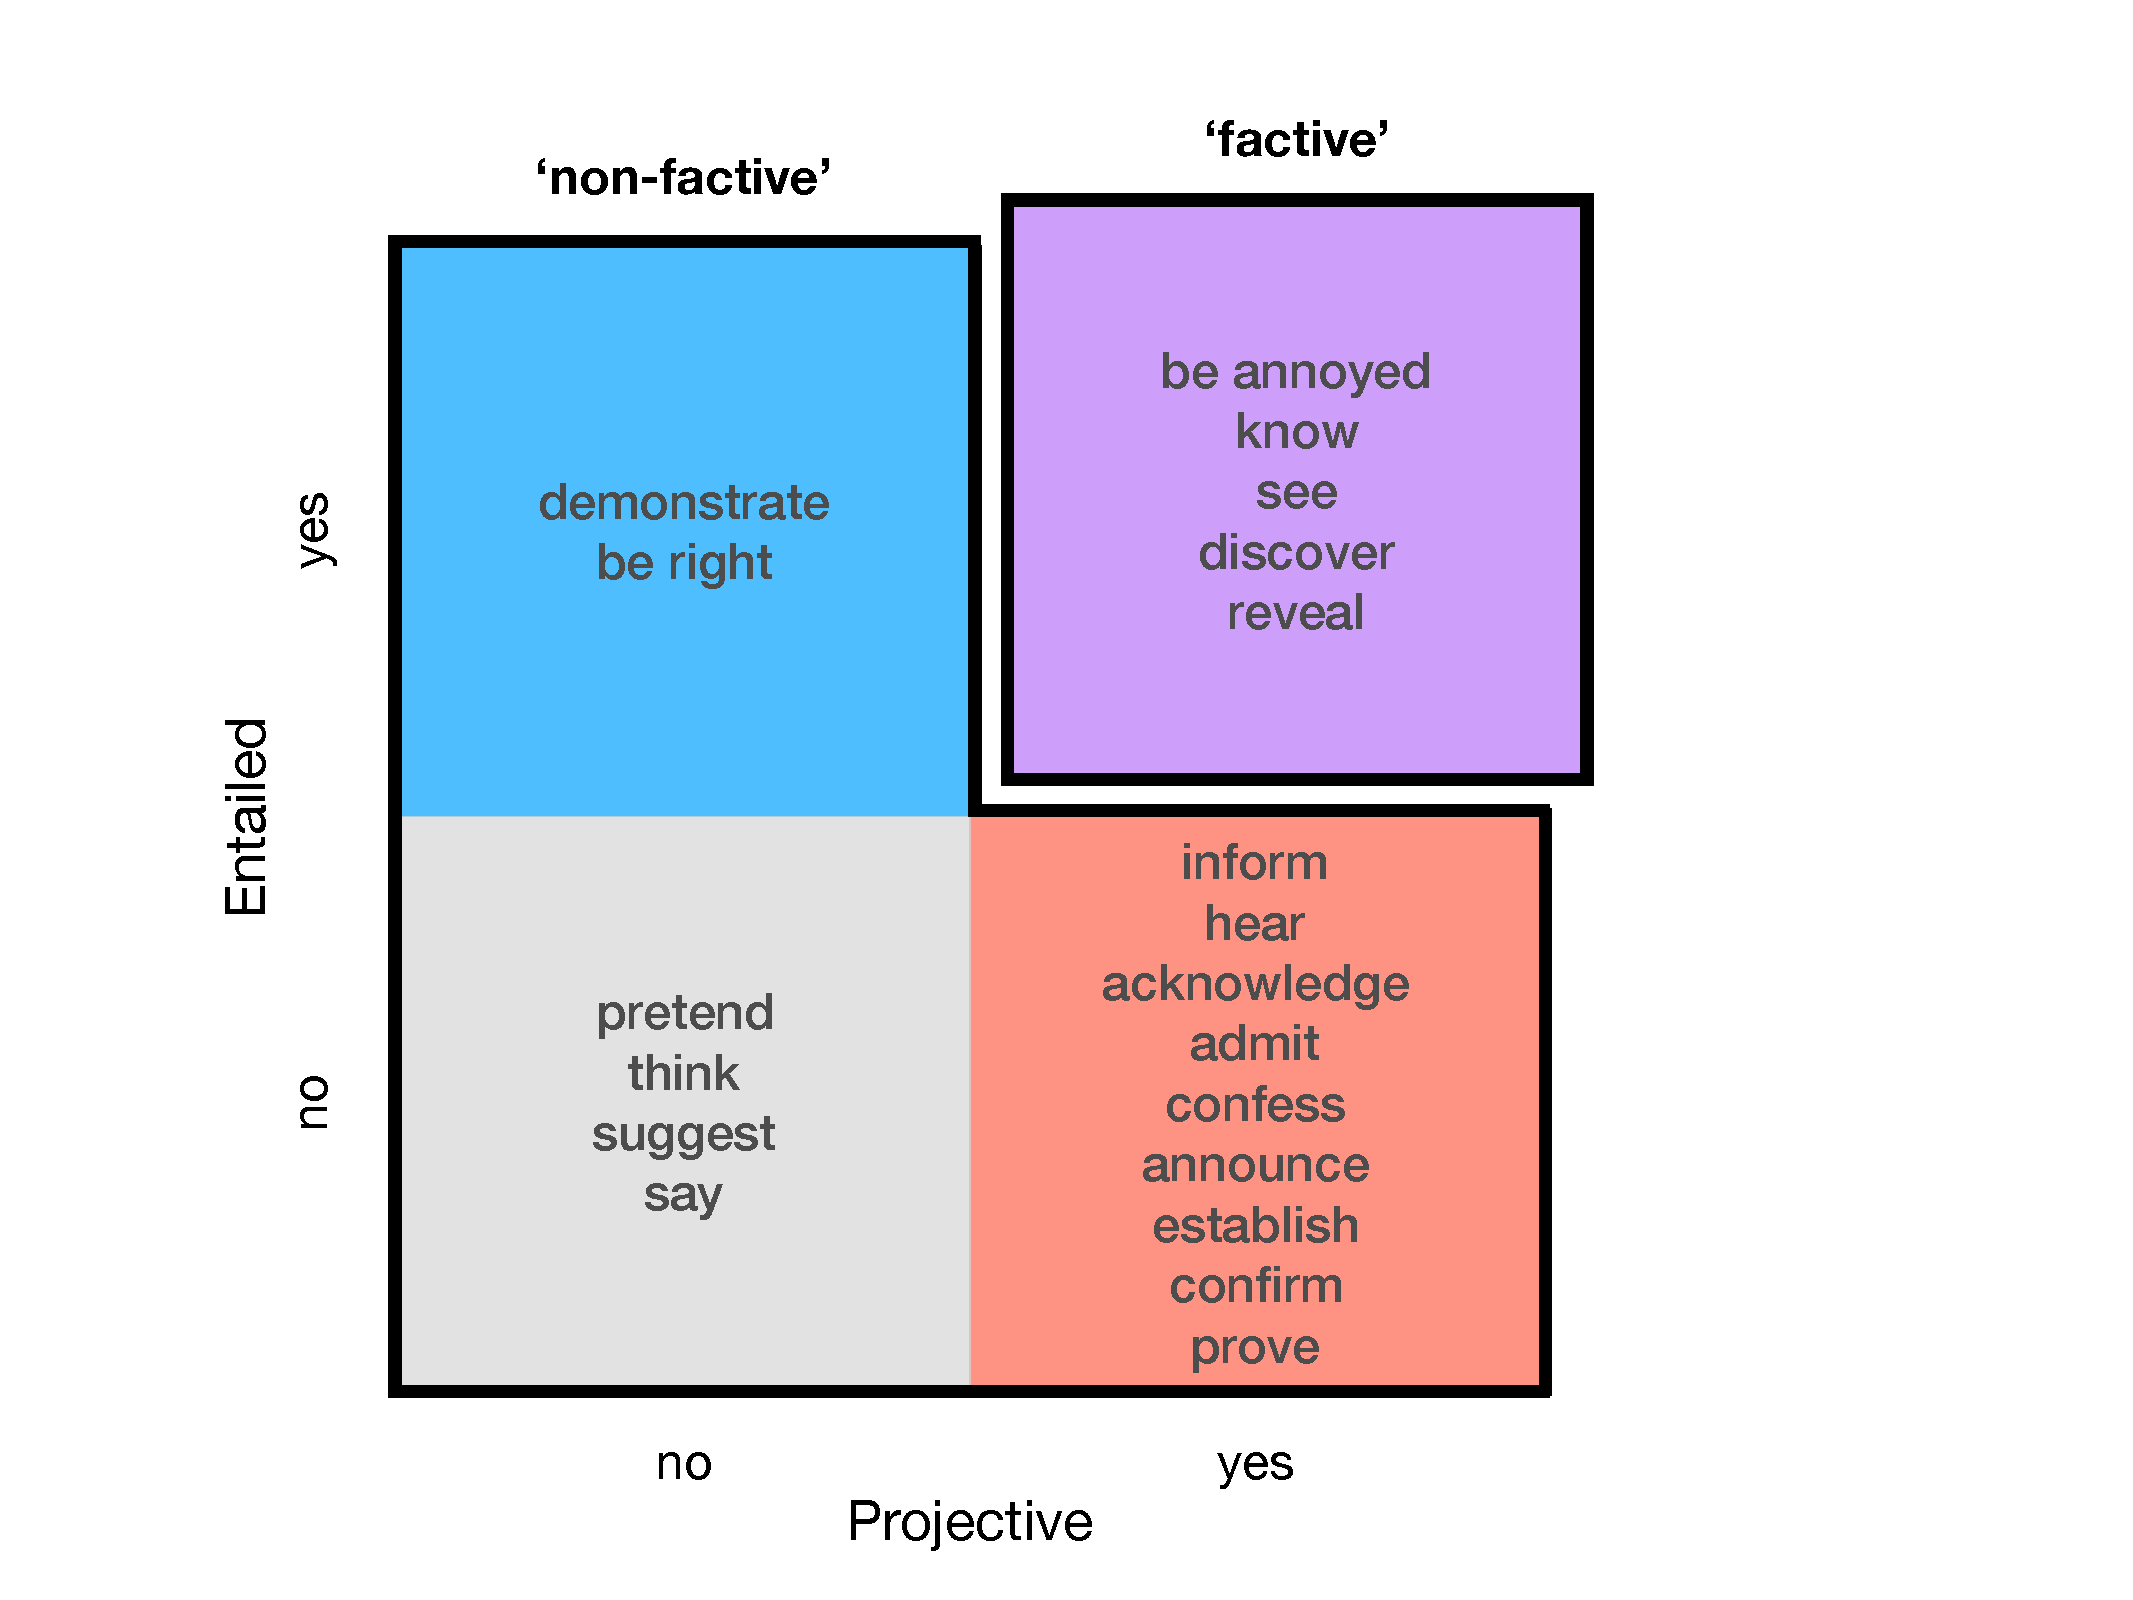
\includegraphics[trim={3.5cm 1cm 7cm 2cm},clip,width=.27\paperwidth]{../paper/figures/categorization}
%%\caption{Assumed categorical classification}
%\end{subfigure} %
%\begin{subfigure}{.3\textwidth}
%\centering
%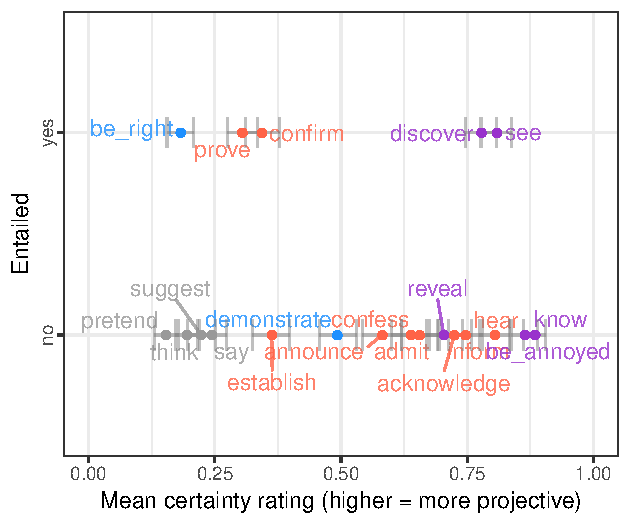
\includegraphics[width=.3\paperwidth]{../results/5-projectivity-no-fact/graphs/projection-by-inferenceEntailment}
%%\caption{Experiment findings}
%\end{subfigure}
%
%\caption{20 English predicates: assumed categorical classification (left panel) vs.\ experiment findings (right panel; mean certainty rating with 95\% CIs, inference diagnostic for entailment.}\label{f-summary-categorical}
%
%\end{figure}

\newpage

\bibliography{../bibliography}

\end{document}
